The previous section showed that dynamically reconfiguring the processor can help reduce energy consumption whilst still achieving the same execution time as the fastest ahead of time configuration.
In order to benefit fully from dynamic core-composition two solutions are possible; either the programmer must go through the code and manually determine when to change the composition or an automatic scheme can be deployed.
This section now presents a learning scheme that is used to exploit the large energy savings available.
The main idea is to monitor at runtime some performance counters and make a decision at a regular interval on how to reconfigure the cores.
For this purpose, a model is trained offline using the data collected and presented earlier in the chapter.
Once trained, the model predicts the optimal number of cores based on the performance counters from the previous time interval and reconfiguration occurs if it is different from the current number of cores.

\begin{figure}[t]
    \centering
	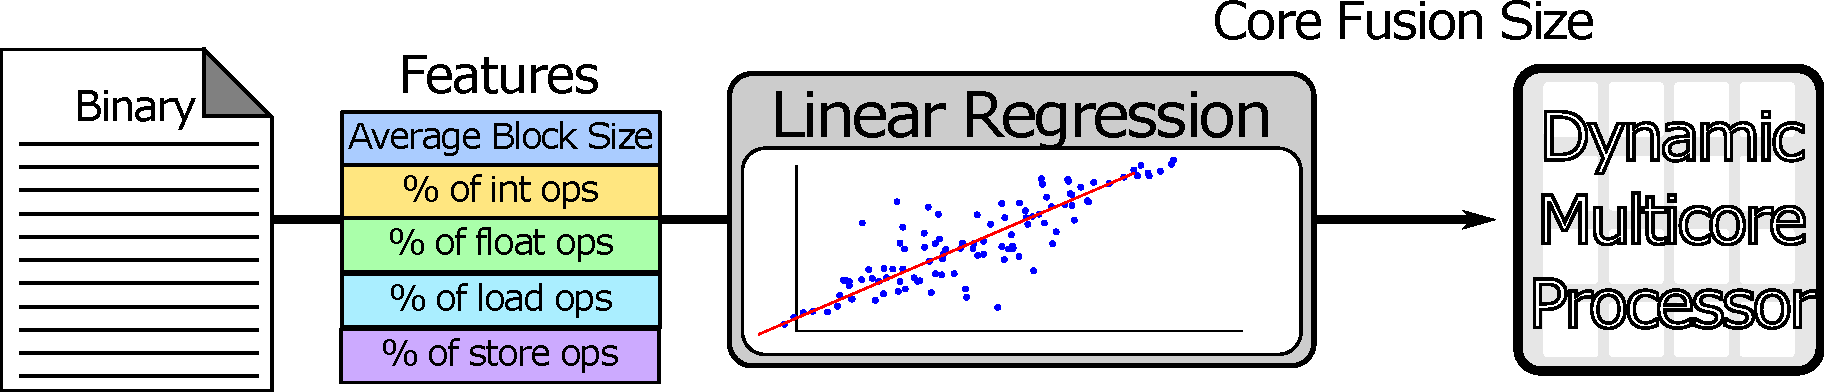
\includegraphics[width=1\textwidth]{cases-paper/graphics/other/model3.pdf}
	\vspace{-2em}
    \caption{Linear Model.}
    \label{fig:linmod}
\end{figure}
\subsection{Model}

As the decisions are made at runtime, a lightweight model that is able to predict the correct configuration that can be integrated in hardware is necessary.
Linear regression, which makes predictions using a weighted sum of the input feature, has been demonstrated to be useful for predicting processor performance~\cite{Joseph2006LinReg}.
It is chosen as it has been as it can easily be implemented in hardware~\cite{lee2006linreg,Lukefahr2012Composite} and has a low overhead when computing the sum.
The model is trained offline using the traces gathered from the prior analysis for the \textbf{DSpeed} scenario which maximises energy savings while maintaining performance.

Figure~\ref{fig:linmod} shows how the linear model is trained.
The dataset consists of a set of four input features (average block size, and percentage of integer, floating point and load operations) and the optimal number of cores for each time tick for each program.
These features are chosen as they are easy to extract from the hardware.
The reason stores are not in the feature vector is due to the fact that a block is comprised only of integer, floating point, load and store operations.
Therefore, when building the model, a correlation analysis determined that stores correlate with other features and selects to remove it as a variable.
 % a single data point is created per phase, averaging the features of all the ticks in a phase, resulting in a total of 34 pairs of optimal core number and features.

To speedup the learning process, for each benchmark the features of all the ticks in a phase were averaged out to create a single data point, which is comprised of an IPC value, and the features described in Figure~\ref{fig:linmod}.
This averaging out leads to 34 data points for all the benchmarks.
The training consists of finding the weights that minimise the error when predicting the optimal number of cores to use across all time ticks and benchmarks.
Since only core configurations which use a power of two number of cores are considered, the linear model is built to predict the logarithm (base 2) of the number of cores.
The prediction is rounded up to the nearest integer in the interval $[0,4]$.
The following equation represents the trained linear model which can be used to make prediction:
\vspace{-1em}
\begin{align*}
  log_2(\textbf{\#cores}) = & -7.7\ +\ 0.028 \cdot \textbf{avgBlkSze}\ +\ 0.075 \cdot \textbf{\%int\_ops}\ +\\
 &0.069 \cdot \textbf{\%fp\_ops}\ +\ 0.21 \cdot \textbf{\%ld\_ops}
\end{align*}

It is important to note that this model was not used during the validation, as cross-validation (see Chapter~\ref{chp:Background}) was used to evaluate it.
Instead, this represents a model where the data from all programs is used.
For instance, if at runtime an average block size of 6 instructions, and 77\%, 1\% and 18\% of integer, floating point and load operations, respectively, then the predicted value will be 2.092.
Rounded up to the nearest integer value, 2, the optimal number of cores predicted will, therefore, be 4.

As can be seen, the largest weight is on the percentage of loads operations.
This is due to different reasons, mainly execution time and the fact that Load-Store Queues are fused.
When it comes to execution time, loads may take from 3 to 128 cycles depending on whether or not it is a cache miss or hit.
Whether it is a cache hit or miss, a block that takes longer to execute will often minimise the \textit{SynchronisationCost} penalty.
A block composed mainly of integer or floating point operations will often result in shorter execution rates; thus may execute faster, making it harder for large logical cores to improve performance.

More discussion on how the time it takes to execute a block influences the performance of core compositions is discussed in Chapter~\ref{chp:hardchanges}.
The other reason loads have the largest weight is due to the fact that loads can be fired independently to the Load-Store Queue.
Unlike stores that depend on previous memory instructions blocks being committed, loads can be fired with less overhead.
As data can be speculatively fetched, load instructions can receive data from other cores before the data is stored, speeding up executions.
By increasing the core count on load heavy blocks this will improve performance more reliably due to cores being able to issue loads in parallel.

\begin{figure}[t]
    \centering
	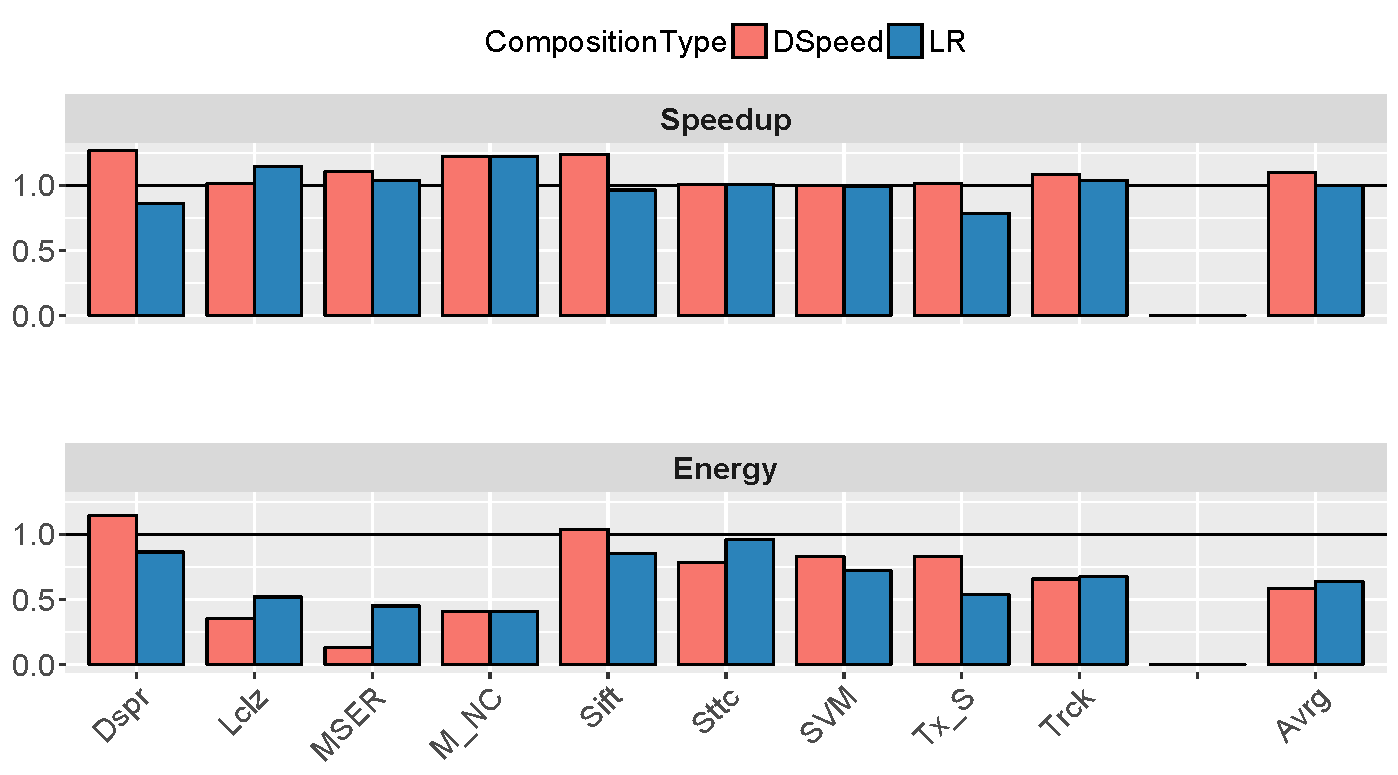
\includegraphics[width=1\textwidth]{cases-paper/graphics/results/lr_speed3.pdf}
    \caption{Performance results for maximising speed for the SD-VBS benchmarks using the linear regression (LR) model. The results are normalised against the Static Suite core composition.}% For Speedup, higher means better, for energy lower is better.}
    \label{fig:speedlr}
	\vspace{1em}
\end{figure}

%explain why MSER here is bad. Most likely because it over-estimates because some features in the vector don't describe the performance in the application.
%This is most likely due to the branch prediction/.
\subsection{Results}

To evaluate the performance of the model leave-one-out cross-validation  is used; it is a standard machine-learning methodology which tests the model using not seen during training.
For instance, if the model is tested for one program, for example \textit{Disparity}, the model is then trained using the dataset from all the other programs combined.
Then the resulting trained linear model is used to predict the optimal core number for each time tick of the disparity program and report the performance achieved.

Figure~\ref{fig:speedlr} shows the performance in terms of speed and energy that is achieved using the linear model normalised by a fixed static configuration.
The fixed configuration maximised performance across all the benchmarks using 8 cores and is the same as in the previous results presented in figure~\ref{fig:speedres}.
On average, the linear regression model is able to consume 37\% less energy compared to the 8 cores fixed configuration and is able to exactly match its speed.
The main outlier is \bm{MSER} where the linear regression consumes over 2x more energy than \textbf{DSpeed}.
This is due to the fact that \bm{MSER} is a benchmark where the branch prediction is poor as previously mentioned in Table~\ref{tab:sd-vbsbpred}.
Indeed, \bm{MSER} has an average branch prediction of 85\% compared to the average of 95\%.S
As \bm{MSER} tends to have very small blocks, the branch prediction makes it very difficult to ever efficiently use even a core composition of size 2.
This benchmark is therefore an outlier compared to the rest of the set, as it is the branch prediction causing incorrect predictions from the linear regression.

The performance is also compared with the best possible choice of dynamic reconfiguration, \textbf{DSpeed} which acts as an Oracle.
As can be seen, the linear model is able to exploit similar energy savings to the \textbf{Dspeed} scheme in most cases.
On average it reduces energy by 37\%, which is within 5 percentage points of the 42\% achievable by the \textbf{Dspeed} scheme.
These results show that it is possible to implement a simple realistic lightweight scheme which offers large energy savings.
